\section{Baseline I/O Performance} \label{sec:results}

\begin{figure}[t]
    \centering
    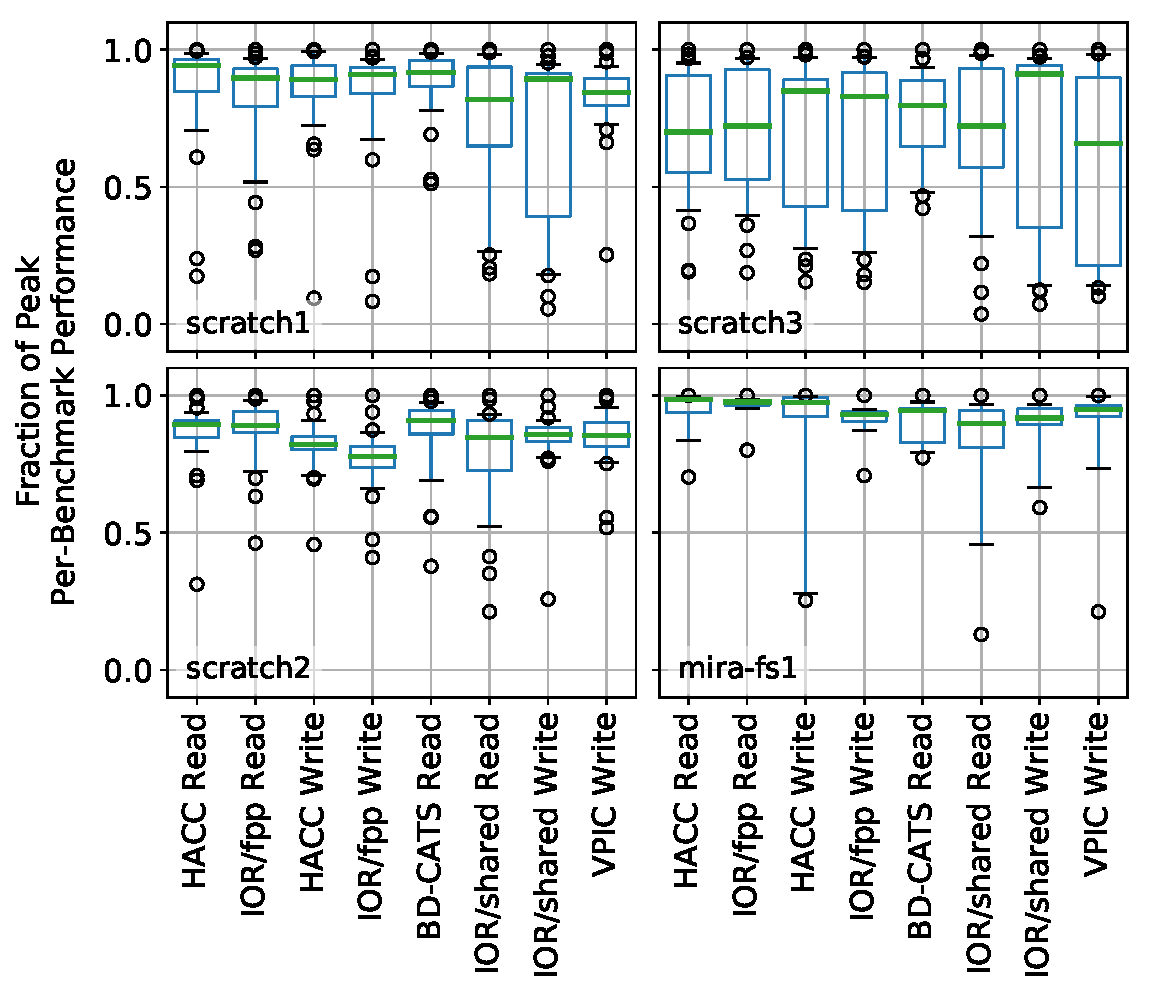
\includegraphics[width=1.0\columnwidth]{figs/perf-boxplots.pdf}
    \vspace{-.25in}
    \caption{I/O performance for all file systems tested grouped by test
    applications and read(R)/write(W) mode.  Whiskers represent the 5th and 95th
    percentiles.}
    \label{fig:perf-summary-boxplots-motif}
	\vspace{-.3in}
\end{figure}

Because variation in peak I/O performance is known to be caused by different I/O access patterns~\cite{Lofstead2010,Uselton2010,Xie2012}, we first establish the baseline variation of each benchmark on each system.
We define the \emph{fraction of peak performance} as the mean I/O bandwidth (performance) of a job divided by the maximum performance observed for all jobs \emph{of the same I/O motif} as listed in Table \ref{tab:bench-config} and whether the job did reads or writes.
For example, the fraction peak performance for a HACC write test is normalized to the highest performance of any HACC write test on the same file system.

The distribution of fraction peak performance, shown in Figure~\ref{fig:perf-summary-boxplots-motif}, reveals that the degree of variation \emph{within} each application varies with each file system.
For example, the HACC write workload is susceptible to a long tail of performance loss on mira-fs1 despite mira-fs1's overall lower variation as evidenced by the distance between all I/O motifs' whiskers relative to the Edison file systems.
Edison's scratch3 also demonstrates broad performance variation for the VPIC write workload, contrasting with the relatively narrow performance variation of this application on other systems.

We conclude that performance variability is the result of factors intrinsic to both the application and the file system;
different I/O motifs result in different levels of performance \emph{and} variability.
Furthermore, these behaviors are not a function of the parallel file system architecture; all Edison file systems are Lustre-based, yet Figure~\ref{fig:perf-summary-boxplots-motif} shows a marked difference in variability between scratch1/scratch2 and scratch3.
Thus, these differences in performance variation must be a function of their different hardware configurations, their specific I/O patterns, or a combination of both.
This finding underscores the importance of examining multiple sources of I/O characterization data (e.g., application-level and server-side) in concert in order to develop a full understanding of I/O performance.

%%%%%%%%%%%%%%%%%%%%%%%%%%%%%%%%%%%%%%%%%%%%%%%%%%%%%%%%%%%%%%%%%%%%%%%%%%%%%%%%
\section{Integrated Analysis} \label{sec:results/umami}
%%%%%%%%%%%%%%%%%%%%%%%%%%%%%%%%%%%%%%%%%%%%%%%%%%%%%%%%%%%%%%%%%%%%%%%%%%%%%%%%

With an understanding of the baseline performance variation on each system and application tested, we then combined application performance data from the sources described in Section \ref{sec:methods} to better understand how performance is affected by extrinsic factors.
Bandwidth contention from other jobs is an intuitive source of performance variation, so we define the \emph{bandwidth coverage factor} ($\mathit{CF}_{\mathit{bw}}$) of a job $j$ to quantify the effects of such competing I/O traffic:

\begin{equation} \label{eq:cf}
    \mathit{CF}_{\mathit{bw}}(j) = \frac{N_{\textup{bytes}}^{\textup{Darshan}}(j)}
    {\sum_{t,s}^{\textup{time,servers}}
    \left [ N_{\textup{bytes}}^{\textup{LMT,ggiostat}}(t,s) \right ] , }
\end{equation}
%
where 
$N_{\textup{bytes}}^{\textup{Darshan}}$ are the bytes read and written by job $j$ according to its Darshan log and 
$N_{\textup{bytes}}^{\textup{LMT,ggiostat}}$ are the bytes read and written to a parallel file system server $s$ during a 5-second time interval $t$.
The time interval over which the job ran ($\mathit{time}$) and the servers to which the job wrote ($\mathit{servers}$) are also stored in the job's Darshan log~\cite{snyder2016modular}.
$\mathit{CF}_{\mathit{bw}}$ is a direct reflection of how much I/O traffic a job competed against in the underlying file systems.
When $\mathit{CF}_{\mathit{bw}} = 1.0$, all the server-side I/O can be attributed to job $j$, whereas $\mathit{CF}_{\mathit{bw}} = 0.5$ indicates that only half of the server-side I/O is attributable to job $j$ while the other half is from other sources.

$\mathit{CF}_{\mathit{bw}}$ can be generalized to any metric for which the contribution of an individual job can be distinguished from the system-level aggregate.
As such, we also define $\mathit{CF}_{\mathit{IOPS}}$ of IOPS (derived from Darshan and ggiostat) and $\mathit{CF}_{\mathit{nodehrs}}$ of node-hours (derived from job-scheduling data).

%In practice, $\mathit{CF}$ can be slightly greater than $1.0$ as a result of two conditions:
%a) when the storage system traffic monitoring (LMT/ggiostat) does not capture data from all servers during a polling interval, or
%b) when clock skew between the compute nodes and the file system servers causes the Darshan log and LMT/ggiostat to have an inconsistent understanding of when I/O happened.
%In this study, such noise never resulted in $\mathit{CF} > 1.2$.
%%%% GKL: The ratio of CF > 1.2 to all CF measurements is very high on Mira; 96 of the 214 measurements provided by Shane were dropped due to this filter criterion

These $\mathit{CF}$ metrics, system health data, and job topology data let us contextualize performance anomalies and quantify where a job's I/O performance falls on the spectrum of normalcy relative to jobs with similar motifs.
To concisely display this information and identify metrics that most likely contribute to abnormal performance, we propose a unified monitoring and metrics interface (UMAMI) diagram as demonstrated in Figure \ref{fig:umami-scratch2-hacc-write}.
UMAMI presents historic measurements (the I/O climate) alongside a box plot that summarizes each metric.
These time series plots terminate at a job of interest and define the I/O weather at the time that job ran.

Overlaying this weather on the climate (dashed lines in the box plots) shows how each metric compares with the distribution of past weather conditions, enabling rapid, holistic differentiation of rare events from long-term performance problems.
In the remainder of this section
we use UMAMI diagrams to identify different factors that do and do not contribute to I/O performance loss.
Although these findings are presented as specific case studies on Mira and Edison, we stress that UMAMI draws data from any component-level monitoring that a system may run at an HPC center.
Hence, these analyses can be easily performed and delivered to users of production HPC systems in a straightforward fashion.

%%%%%%%%%%%%%%%%%%%%%%%%%%%%%%%%%%%%%%%%%%%%%%%%%%%%%%%%%%%%%%%%%%%%%%%%%%%%%%%%
\subsection{Case study: I/O contention}
%%%%%%%%%%%%%%%%%%%%%%%%%%%%%%%%%%%%%%%%%%%%%%%%%%%%%%%%%%%%%%%%%%%%%%%%%%%%%%%%

\begin{figure}[t]
    \centering
    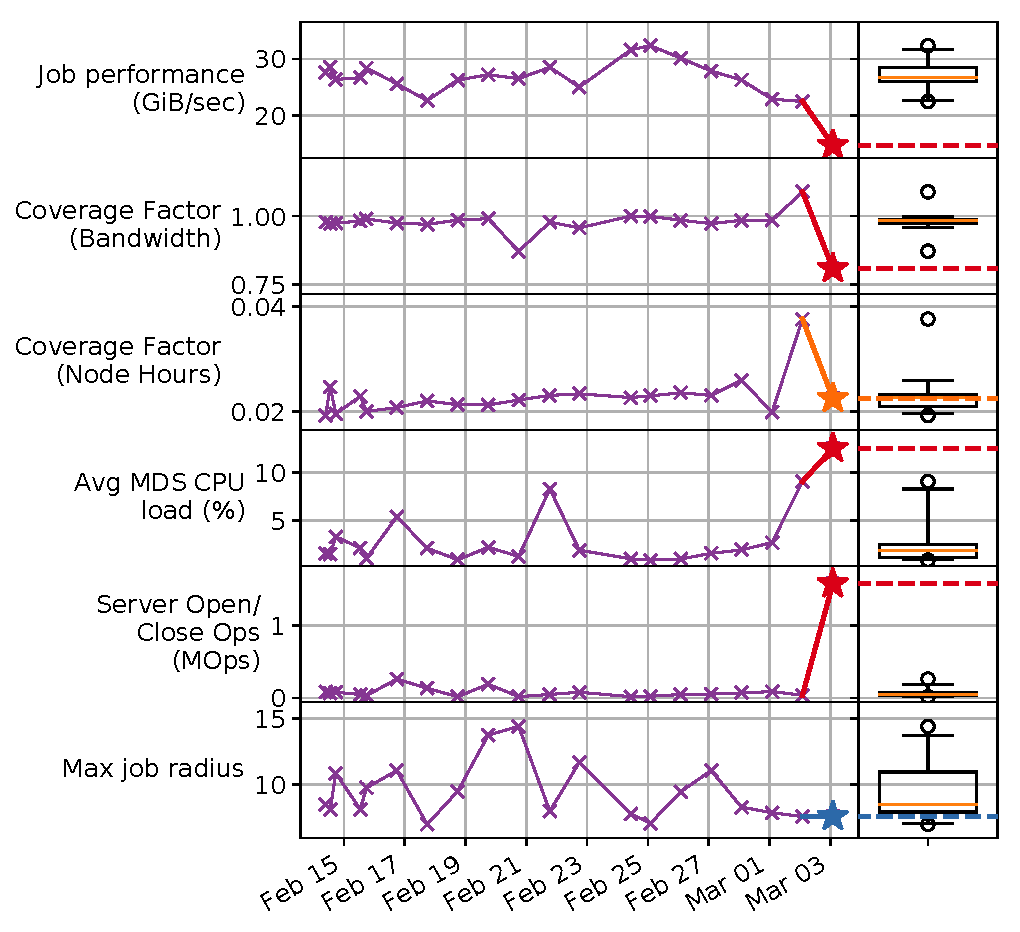
\includegraphics[width=1.0\columnwidth]{figs/umami-scratch2-hacc-write.pdf}
    \vspace{-.25in}
    \caption{UMAMI of HACC write workloads on the Edison scratch2 file system.
    Left panes show the measurements from previous runs of the same motif; right panes summarize the distribution of these metrics.
    The star denotes the metrics for the most recent job and is colored according to the quartile in which it falls (red being the worst quartile and blue the best).
    Whiskers indicate 5th and 95th percentiles; outliers are circles.}
    \label{fig:umami-scratch2-hacc-write}
    \vspace{-.2in}
\end{figure}

The UMAMI example in Figure \ref{fig:umami-scratch2-hacc-write} represents a HACC write test whose "Job performance" measurement and its value relative to previous instances of this type of job indicate statistically abnormal performance.
This poor performance was accompanied by an unusually low $\mathit{CF}_{\mathit{bw}}$ and high metadata load, highlighted as red dashed lines in the box plots that denote their place in the least-favorable quartile of past measurements.
The metrics corresponding to orange dashed lines ($\mathit{CF}_{\mathit{nodehrs}}$ and the number of overlapping jobs) fall in the second quartile, indicating that the number of concurrently running jobs and concurrently active compute nodes are too coarse-grained a metric to predict I/O performance.
The metric corresponding to blue dashed line, the maximum job radius, falls into the most favorable quartile for this problematic job, and HACC has shown good I/O performance on much more topologically distributed node allocations.
Thus, HACC job's poor performance was a result of I/O loads extrinsic to this job that competed for both bandwidth and metadata operation rates; the number of concurrently running jobs and HACC's placement on the dragonfly network had no clear impact.

%%%%%%%%%%%%%%%%%%%%%%%%%%%%%%%%%%%%%%%%%%%%%%%%%%%%%%%%%%%%%%%%%%%%%%%%%%%%%%%%
\subsection{Case study: metadata load}
%%%%%%%%%%%%%%%%%%%%%%%%%%%%%%%%%%%%%%%%%%%%%%%%%%%%%%%%%%%%%%%%%%%%%%%%%%%%%%%%

\begin{figure}[t]
    \centering
    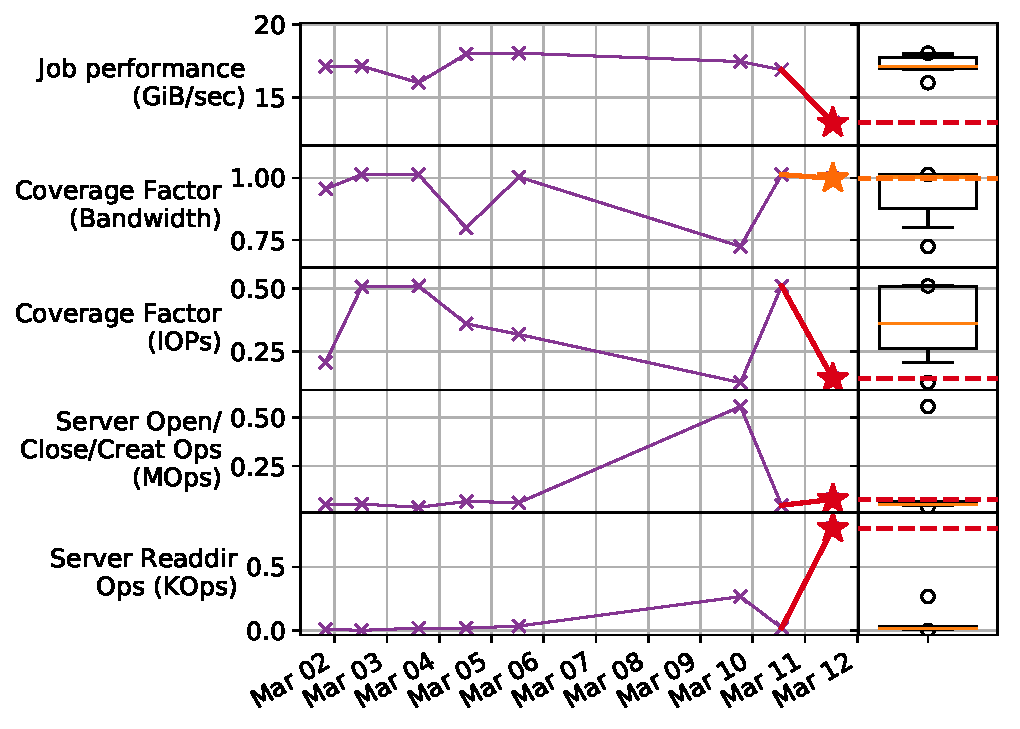
\includegraphics[width=1.0\columnwidth]{figs/umami-mira-fs1-vpic-write.pdf}
    \vspace{-.25in}
    \caption{UMAMI demonstrating the climate surrounding VPIC-IO write workloads on Mira compared with a most recent run, which showed highly unusual weather in the form of an excess of \texttt{readdir(3)} calls.
%   Significance of each pane and its contents are the same as explained in Figure \ref{fig:umami-scratch2-hacc-write}.
    }
    \label{fig:umami-mira-fs1-vpic-write}
	\vspace{-.15in}
\end{figure}

Figure \ref{fig:umami-mira-fs1-vpic-write} shows the UMAMI for a poorly performing VPIC workload.
$\mathit{CF}_{\mathit{bw}}$ is within normal parameters, indicating normal (minimal) levels of bandwidth contention.
$\mathit{CF}_{\mathit{IOPS}}$ is abnormally low, although previous values have been equally low despite a lack of dramatic performance loss (e.g., on March 4 and March 9).
The only metric that shows a unique, undesirable value is the number of \texttt{readdir(3)} operations handled by the file system, indicative of an expansive file system traversal that was being performed at the same time as the job execution.   From this, we can infer that a namespace scan, not bandwidth contention, contributed to the abnormally poor HACC performance on the March 11 run.

%%%%%%%%%%%%%%%%%%%%%%%%%%%%%%%%%%%%%%%%%%%%%%%%%%%%%%%%%%%%%%%%%%%%%%%%%%%%%%%%
\subsection{Case study: storage capacity}
%%%%%%%%%%%%%%%%%%%%%%%%%%%%%%%%%%%%%%%%%%%%%%%%%%%%%%%%%%%%%%%%%%%%%%%%%%%%%%%%

\begin{figure}[t]
    \centering
    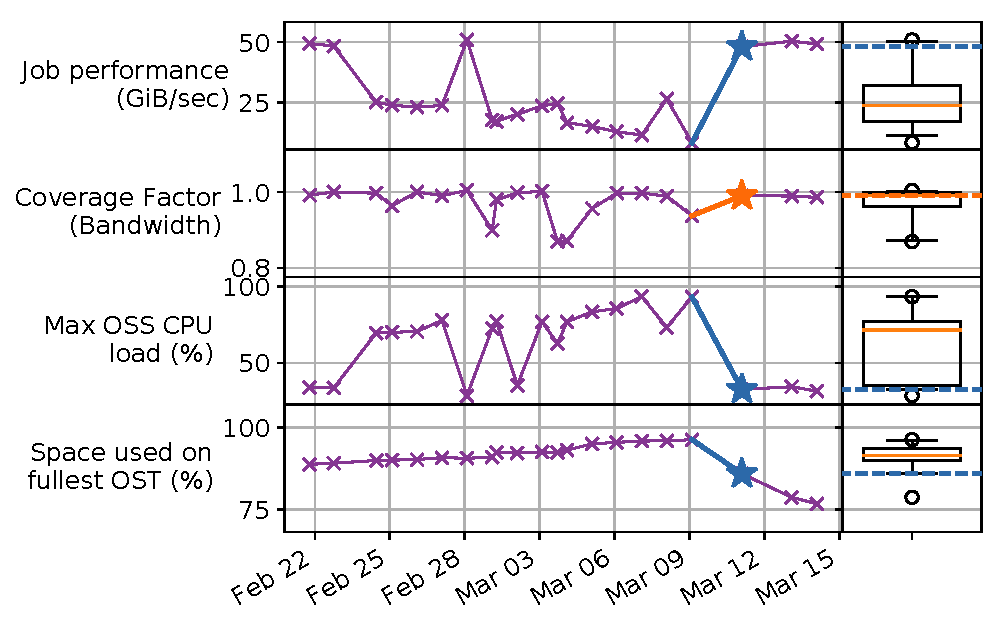
\includegraphics[width=1.0\columnwidth]{figs/umami-scratch3-hacc-write-long-term.pdf}
    \vspace{-.25in}
    \caption{UMAMI of HACC write performance on Edison's scratch3 file system showing a longer-term period of performance degradation that was associated with unusually high OSS CPU load.
%   Significance of each pane and its contents are the same as explained in Figure \ref{fig:umami-scratch2-hacc-write}.
    }
    \label{fig:umami-scratch3-hacc-write-long-term}
	\vspace{-.15in}
\end{figure}

This holistic approach can also identify longer-term performance degradation.
Figure \ref{fig:umami-scratch3-hacc-write-long-term} shows the UMAMI view of Edison's scratch3 file system when coverage factors were not unusual despite an ongoing $2\times$ slowdown over the normal 50 GiB/sec between February 24 and March 9.
The magnitude of performance loss closely followed the maximum CPU load observed on the Lustre OSSes, and this period also coincided with the scratch3 file system reaching critical levels of fullness.
A file system purge at NERSC, initiated on March 9, then resulted in restored I/O performance for the last three jobs shown.
This relationship between CPU load and I/O performance points to an increasing cost of scavenging empty blocks on writes, and this behavior is consistent with known performance losses that result from Lustre OSTs filling~\cite{oral2014best}.  
